\section{例题与分析}

\begin{question}
\begin{example}[经过狭缝观察米尺]\label{ex:ho1}
平面镜 $AB$、水平放置的米尺 $P_1P_2$ 与不透明屏 $MN$ 相互平行。屏上 $ab$ 为透光狭缝，米尺有刻度的一面朝向镜面。眼睛紧贴米尺上的小孔 $S$，位置如图\ref{fig:ho1q}。用作图法确定能经平面镜看到的米尺部分。
\end{example}
\fig{fig:ho1q}{反射前后两段光路均须穿过狭缝 $ab$。各段长度未给出，按几何作图确定范围。}{
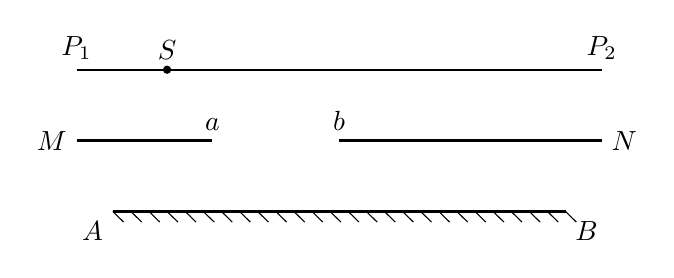
\begin{tikzpicture}[x=1.15cm,y=.9cm]
\draw[thick](-.4,2)--(5.4,2);\node[above]at(-.4,2){$P_1$};\node[above]at(5.4,2){$P_2$};
\fill(.6,2)circle(1.5pt)node[above]{$S$};
\draw[very thick](-.4,1)--(1.1,1) (2.5,1)--(5.4,1);
\node[left]at(-.4,1){$M$};\node[right]at(5.4,1){$N$};\node[above]at(1.1,1){$a$};\node[above]at(2.5,1){$b$};
\draw[very thick](0,0)--(5,0);\foreach \x in {0,.2,...,5}{\draw(\x,0)--({\x+.12},-.15);}
\node[below left]at(0,0){$A$};\node[below right]at(5,0){$B$};
\end{tikzpicture}}
\end{question}

\begin{solution}\textbf{把眼点与两次穿缝条件展开到同一直线}\par\nobreak
先在图\ref{fig:ho1s}中把眼睛 $S$ 对镜面对称为 $S'$，再把狭缝端点 $a,b$ 对称为 $a',b'$。任取米尺上的点 $Q$，若反射点为 $P$，把反射段 $P\to S$ 展开，整条光路便成为直线 $Q\to P\to S'$。

这条直线必须依次通过三个允许区域：实狭缝 $ab$、镜段 $AB$、虚狭缝 $a'b'$。实狭缝限制入射段 $Q\to P$，虚狭缝限制折回后的 $P\to S$。因此应作 $S'a,S'b$、$S'a',S'b'$、$S'A,S'B$ 并延长到米尺所在直线；三组线各给出一个允许区间，再与米尺本身取交集。
\fig{fig:ho1s}{镜像展开同时保留实、虚狭缝。粗米尺段 $Q_-Q_+$ 是各允许区间的交集。}{
\begin{tikzpicture}[x=1.15cm,y=.85cm]
\draw(-.4,2)--(5.4,2);\draw[very thick](2.6,2)--(3.13333,2);
\draw[very thick](-.4,1)--(1.1,1) (2.5,1)--(5.4,1);\draw[thick](0,0)--(5,0);
\draw[aux](-.4,-1)--(1.1,-1) (2.5,-1)--(5.4,-1);
\draw[virtual](.6,-2)--(2.6,2) (.6,-2)--(3.13333,2);
\fill(.6,-2)circle(1.5pt)node[below]{$S'$};\node[above]at(.6,2){$S$};
\node[above left]at(1.1,1){$a$};\node[above right]at(2.5,1){$b$};
\node[below left]at(1.1,-1){$a'$};\node[below right]at(2.5,-1){$b'$};
\node[above left]at(2.6,2){$Q_-$};\node[above right]at(3.13333,2){$Q_+$};
\node[below left]at(0,0){$A$};\node[below right]at(5,0){$B$};
\end{tikzpicture}}



\par\medskip\Needspace{4\baselineskip}\noindent\textbf{折回两条边界线，检查实际反射路径}\par\nobreak
图\ref{fig:ho1s}所示位置中，左边界由 $S'a'$ 与米尺的交点 $Q_-$ 决定，右边界由 $S'b$ 的交点 $Q_+$ 决定。

将两条边界线在镜面处折回，得到图\ref{fig:ho1path}；可直接检查两段光线都经过 $ab$，且两个反射点都在 $AB$ 内。
\fig{fig:ho1path}{两条边界的实际反射光路。左边界的返回段擦过 $a$，右边界的入射段擦过 $b$。}{
\begin{tikzpicture}[x=1.15cm,y=.95cm]
\draw(-.4,2)--(5.4,2);\draw[very thick](2.6,2)--(3.13333,2);
\draw[very thick](-.4,1)--(1.1,1) (2.5,1)--(5.4,1);\draw[very thick](0,0)--(5,0);
\draw[ray](2.6,2)--(1.6,0);\draw[ray](1.6,0)--(.6,2);
\draw[ray](3.13333,2)--(1.86667,0);\draw[ray](1.86667,0)--(.6,2);
\node[above]at(.6,2){$S$};\node[above left]at(2.6,2){$Q_-$};\node[above right]at(3.13333,2){$Q_+$};
\node[above left]at(1.1,1){$a$};\node[above right]at(2.5,1){$b$};\node[below]at(1.6,0){$P_-$};\node[below right]at(1.86667,-.3){$P_+$};\draw[aux](1.86667,0)--(1.86667,-.3);
\end{tikzpicture}}


\par\medskip\Needspace{4\baselineskip}\noindent\textbf{写出镜面和两次穿屏的交点坐标}\par\nobreak
还可用坐标核对作图。设镜面 $y=0$，米尺 $y=D$，屏 $y=h$，$0<h<D$，眼睛横坐标为 $s$，物点横坐标为 $q$。镜面交点与两次穿屏点分别为
\[
x_P=\frac{q+s}{2},\quad
x_{\text{入}}=s+\frac{D+h}{2D}(q-s),\quad
x_{\text{回}}=s+\frac{D-h}{2D}(q-s).
\]
同时要求 $x_P\in[A,B]$、$x_{\text{入}},x_{\text{回}}\in[a,b]$，并令 $q\in[P_1,P_2]$，所得正是上述交集。只检查一次穿缝会把不可见部分也算进去。



\par\medskip\Needspace{4\baselineskip}\noindent\textbf{把各通光限制化为同一米尺上的区间}\par\nobreak
图\ref{fig:ho1intervals}将三组投影区间并列画出，各行横坐标对应同一个米尺位置。沿竖线比较各行，便可找出公共部分。仍用 $a,b,A,B$ 表示相应端点的横坐标，前三组范围分别为
\begin{align*}
I_{\text{入}}&=\left[s+\frac{2D(a-s)}{D+h},\ s+\frac{2D(b-s)}{D+h}\right],\\
I_{\text{回}}&=\left[s+\frac{2D(a-s)}{D-h},\ s+\frac{2D(b-s)}{D-h}\right],\\
I_{\text{镜}}&=[2A-s,\ 2B-s].
\end{align*}
\fig{fig:ho1intervals}{将三种通光限制投影到米尺所在直线后，取它们与米尺的公共部分。各行横向尺度相同。}{
\begin{tikzpicture}[x=.7cm,y=.8cm]
\foreach \y/\txt in {3/实狭缝,2/返回狭缝,1/有限镜段,0/米尺}{\draw[black!30](-.6,\y)--(9.4,\y);\node[left]at(-1,\y){\txt};}
\draw[line width=1.2pt](1.266667,3)--(3.133333,3);\draw[line width=1.2pt](2.6,2)--(8.2,2);\draw[line width=1.2pt](-.6,1)--(9.4,1);\draw[line width=1.2pt](-.4,0)--(5.4,0);
\draw[aux](2.6,-.3)--(2.6,3.3) (3.133333,-.3)--(3.133333,3.3);\draw[line width=2.2pt](2.6,-.75)--(3.133333,-.75);
\node[below left]at(2.6,-.75){$Q_-$};\node[below right]at(3.133333,-.75){$Q_+$};\node[left]at(-1,-.75){可见部分};
\end{tikzpicture}}


\par\medskip\Needspace{4\baselineskip}\noindent\textbf{取交集并说明控制边界随摆放改变}\par\nobreak
所求为 $I_{\text{入}}\cap I_{\text{回}}\cap I_{\text{镜}}\cap[P_1,P_2]$。若另换眼睛或狭缝位置，控制左右边界的限制可能改变，甚至使交集为空；因而图\ref{fig:ho1s}中的 $S'a'$ 与 $S'b$ 是该示意位置下的控制线，并非所有摆放方式都由这两条线控制。

\end{solution}

\begin{question}
\begin{example}[夹角镜中的像数]\label{ex:ho2}
两个平面镜的夹角分别为 $45^\circ,60^\circ,120^\circ$，物体均放在夹角平分线上。分别求像的个数。镜面足够大，忽略遮挡，见图\ref{fig:ho2q}。
\end{example}
\fig{fig:ho2q}{物体 $S$ 在两镜的角平分线上。反复镜像保持到交点 $O$ 的距离。}{
\begin{tikzpicture}
\draw[very thick](0,0)--(4,0) (0,0)--(2,3.464);
\draw[aux](0,0)--(30:3.5);\fill(30:2.2)circle(1.8pt)node[above]{$S$};
\draw(.7,0)arc(0:60:.7);\node at(1,.55){$\alpha$};\node[below left]at(0,0){$O$};
\end{tikzpicture}}
\end{question}

\begin{solution}\textbf{反复镜像并按圆周位置去重}\par\nobreak
依次把 $S$ 对两镜作对称，每个像仍位于以 $O$ 为圆心、$OS$ 为半径的圆上。本题中 $m=360^\circ/\alpha$ 分别为8、6、3，物体又位于角平分线上，反复镜像恰好得到 $m$ 个不同位置，分布在等分扇区的中线上。绕满一周后与已有位置重合，计数便应停止。
\fig{fig:ho2s}{实心点为物体，空心点为不同的像。三种情况下均须从圆周总位置数中扣除物体本身。}{
\begin{tikzpicture}[scale=.8]
\foreach \xx/\aa/\mm in {0/45/8,4.7/60/6,9.4/120/3}{
\begin{scope}[shift={(\xx,0)}]
\draw[aux](0,0)circle(1.65);\draw[thick](0,0)--(0:2) (0,0)--(\aa:2);
\pgfmathsetmacro{\half}{\aa/2}
\foreach \k in {0,...,\numexpr\mm-1\relax}{
\pgfmathsetmacro{\ang}{\half+\k*\aa}
\ifnum\k=0\fill(\ang:1.65)circle(1.8pt);\node at(\ang:2.12){$S$};
\else\draw[fill=white](\ang:1.65)circle(1.8pt);\fi}
\node[below]at(0,-2.2){$\alpha=\aa^\circ$};
\end{scope}}
\end{tikzpicture}}



\par\medskip\Needspace{4\baselineskip}\noindent\textbf{扣除物点，分别得到三种像数}\par\nobreak
图\ref{fig:ho2s}分别有8、6、3个不同位置，其中一个是真实物体，故
\[
\boxed{N_{45^\circ}=7,\qquad N_{60^\circ}=5,\qquad N_{120^\circ}=2.}
\]
也可核对 $120^\circ$ 的情形：物体在 $60^\circ$ 方向，对下镜反射到 $300^\circ$，对上镜反射到 $180^\circ$；再反射只会回到这三个位置。

物体位于角平分线是这个计数的条件，不能把同一简式不加判断地用于任意物体位置或任意夹角。

这里数的是不同的像位置，不能按“反射了几次”累计。图\ref{fig:ho2s}每个空心点都可由一串镜像得到，另一串镜像若落到同一点，就不再增加像数。对 $45^\circ$、$60^\circ$，位置方向可依次写成 $\alpha/2+k\alpha$；$k$ 达到 $m$ 时回到起点。这解释了为何要在 $m$ 个位置中扣除真实物体，并在闭合后停止。



\par\medskip\Needspace{4\baselineskip}\noindent\textbf{检查镜面大小和观察窗口的附加限制}\par\nobreak
应将像的位置计数与具体眼点能看见哪些像分开。前者按图\ref{fig:ho2s}的镜像位置去重；后者还要从眼点向像连线，检查各次反射是否落在实际镜面上。本题已约定镜面足够大且忽略遮挡，因此求的是给定镜角和物体位置下的像数；若另给有限镜长或观察窗口，就必须增加可见光路的筛选。
\end{solution}

\begin{question}
\begin{example}[小夹角镜间的反复反射]\label{ex:ho3}
两镜 $L_1,L_2$ 相交于 $O$，夹角 $\alpha=15^\circ$，$A$ 在 $L_2$ 上，$OA=10\,\mathrm{cm}$。从 $A$ 沿垂直于 $L_2$ 的方向发出光线，先射向 $L_1$，此后反复反射，直到平行于某一镜面射出。求从 $A$ 到最后一次反射点的总路程，见图\ref{fig:ho3q}。
\end{example}
\fig{fig:ho3q}{两镜朝右张开，起始光线垂直于下镜。}{
\begin{tikzpicture}[scale=1.4]
\draw[very thick](0,0)--(4.6,0)node[right]{$L_2$};\draw[very thick](0,0)--(4.6,{4.6*tan(15)})node[right]{$L_1$};
\draw[ray](1,0)--(1,{tan(15)});\fill(1,0)circle(1.4pt)node[below]{$A$};\node[below left]at(0,0){$O$};
\draw[dim](0,-.45)--(1,-.45)node[midway,below]{$10\,\mathrm{cm}$};\draw(.6,0)arc(0:15:.6);\draw[aux](.7,.09)--(1.3,.55);\node[above]at(1.3,.55){$15^\circ$};
\end{tikzpicture}}
\end{question}

\begin{solution}\textbf{逐次计算传播方向，确定最后反射点}\par\nobreak
在图\ref{fig:ho3s}中，依次记反射点为 $P_1,\ldots,P_5$。用相对下镜的方向角计算，每次在上镜反射取 $\theta_{\text{出}}=30^\circ-\theta_{\text{入}}$，每次在下镜反射取 $\theta_{\text{出}}=-\theta_{\text{入}}$，得到
\[
90^\circ\to-60^\circ\to60^\circ\to-30^\circ\to30^\circ\to0^\circ.
\]
因此共有5次反射，最后在上镜的 $P_5$ 处反射后平行于 $L_2$ 射出。


\par\medskip\Needspace{4\baselineskip}\noindent\textbf{用当地法线核对五次碰撞的入射角}\par\nobreak
这里的 $\theta$ 是传播方向相对水平轴的角，不是入射角。若改从各点法线量起，图\ref{fig:ho3s}中五次碰撞的入射角分别为
\[
\begin{array}{c|ccccc}
\text{碰撞点}&P_1&P_2&P_3&P_4&P_5\\\hline
i&15^\circ&30^\circ&45^\circ&60^\circ&75^\circ
\end{array}
\]
第一段光线垂直下镜，却斜入射到上镜，故在 $P_1$ 的入射角是 $15^\circ$，并非零。

最后一条水平光线留在两镜间的开口内，不会再碰到下镜。
\fig{fig:ho3s}{五次反射的实际光路。数字按碰撞先后标记，$P_5$ 是最后一次反射点。}{
\begin{tikzpicture}[scale=1.65]
\draw[thick](0,0)--(4.6,0) (0,0)--(4.6,{4.6*tan(15)});
\coordinate(A)at(1,0);\coordinate(P1)at(1,{tan(15)});\coordinate(P2)at(1.154701,0);\coordinate(P3)at(1.366025,.366025);\coordinate(P4)at(2,0);\coordinate(P5)at(3.732051,1);
\draw[ray](A)--(P1);\draw[ray](P1)--(P2);\draw[ray](P2)--(P3);\draw[ray](P3)--(P4);\draw[ray](P4)--(P5);\draw[ray](P5)--(4.6,1);
\node[below left]at(A){$A$};\node[below right]at(P2){$P_2$};\node[below]at(P4){$P_4$};\node[above]at(P5){$P_5$};
\draw[aux](P1)--(.75,.7);\node[above]at(.75,.7){$P_1$};\draw[aux](P3)--(1.7,.85);\node[above]at(1.7,.85){$P_3$};\node[below left]at(0,0){$O$};
\end{tikzpicture}}



\par\medskip\Needspace{4\baselineskip}\noindent\textbf{展开镜区，把五段折线拉直}\par\nobreak
将五段光路展开，可把总路程化为一条线段的长度。每次反射后，把后续镜区翻到前一镜区的另一侧，光路便拉直。图\ref{fig:ho3unfold}中，五个碰撞面依次成为与水平成 $15^\circ,30^\circ,45^\circ,60^\circ,75^\circ$ 的射线；光路始终沿过 $A$ 的竖直线前进。

\fig{fig:ho3unfold}{展开后的同一条直光线。$E$ 是 $P_5$ 的展开位置，$HE=OA$ 为水平尺度，$AE$ 等于实际总路程。}{
\begin{tikzpicture}[scale=1.1]
\foreach \a in {0,15,30,45,60,75}{\draw[black!55](0,0)--(\a:4.1);}
\draw[ray](1,0)--(1,3.732051);\fill(1,3.732051)circle(1.5pt)node[above right]{$E$};
\draw[aux](0,3.732051)--(1,3.732051);\node[left]at(0,3.732051){$H$};
\node[below]at(1,0){$A$};\node[below left]at(0,0){$O$};\node[left]at(.3,1.5){$75^\circ$};
\draw[dim](0,-.35)--(1,-.35)node[midway,below]{$OA$};
\end{tikzpicture}}


\par\medskip\Needspace{4\baselineskip}\noindent\textbf{由直角三角形求总路程并界定终点}\par\nobreak
展开只作刚性反射，故各段长度之和不变。直角三角形 $OAE$ 给出
\[
\boxed{s=AE=OA\tan75^\circ
=10(2+\sqrt3)\,\mathrm{cm}\simeq37.32\,\mathrm{cm}.}
\]
这里计算到 $P_5$ 为止，不包括平行于下镜射出后的路程。
\end{solution}

\begin{question}
\begin{example}[由光路比较折射率]\label{ex:ho4}
光依次穿过平行的介质I、II、III，各段与法线的夹角如图\ref{fig:ho4q}所示。选出所有正确说法：A．介质II是三者中的光密介质；B．介质I的折射率最大；C．介质III的折射率比I大；D．光在介质III中的速度最小。
\end{example}
\fig{fig:ho4q}{两个界面平行，三个角均从法线量起，依次为 $45^\circ,60^\circ,30^\circ$。}{
\begin{tikzpicture}
\fill[black!5](-2,-1.5)rectangle(3.8,0);\fill[black!10](-2,-3)rectangle(3.8,-1.5);
\draw(-2,0)--(3.8,0) (-2,-1.5)--(3.8,-1.5);
\draw[ray](-1.2,1.2)--(0,0);\draw[ray](0,0)--(2.598076,-1.5);\draw[ray](2.598076,-1.5)--(3.290897,-2.7);
\draw[normal](0,1.3)--(0,-1.2) (2.598076,-.3)--(2.598076,-2.8);
\node at(-.45,.8){$45^\circ$};\node at(.55,-.75){$60^\circ$};\node[right]at(2.7,-2.25){$30^\circ$};
\node at(2.5,.6){I};\node at(-1.4,-.7){II};\node at(-1.4,-2.2){III};
\end{tikzpicture}}
\end{question}

\begin{solution}\textbf{用平行界面确定共同折射参数}\par\nobreak
图\ref{fig:ho4s}将三段共用的折射参数记为 $p$。由于界面法线平行，逐面折射给出
\[
n_{\rm I}\sin45^\circ=n_{\rm II}\sin60^\circ
=n_{\rm III}\sin30^\circ=p.
\]
所以
\[
n_{\rm I}=\sqrt2p,\qquad n_{\rm II}=\frac2{\sqrt3}p,
\qquad n_{\rm III}=2p.
\]
\fig{fig:ho4s}{将三段转到同一法线旁比较。共同的 $n\sin\theta$ 使角越小的一段对应折射率越大。}{
\begin{tikzpicture}
\draw[normal](0,0)--(0,-3.2);\draw[ray](0,0)--({3*sin(45)},{-3*cos(45)});
\draw[ray](0,0)--({3*sin(60)},{-3*cos(60)});\draw[ray](0,0)--({3*sin(30)},{-3*cos(30)});
\node[right]at(2.65,-1.5){II，$60^\circ$};\node[right]at(2.15,-2.15){I，$45^\circ$};\node[right]at(1.5,-2.65){III，$30^\circ$};
\node at(-1.3,-1.5){共同法线};
\end{tikzpicture}}



\par\medskip\Needspace{4\baselineskip}\noindent\textbf{比较折射率与光速，判断各选项}\par\nobreak
由此 $n_{\rm III}>n_{\rm I}>n_{\rm II}$，而 $v=c/n$，故 $v_{\rm III}<v_{\rm I}<v_{\rm II}$。答案为 $\boxed{\mathrm C,\mathrm D}$。介质II的折射率最小，是三者中光速最大的一层。
图\ref{fig:ho4q}第一界面处，光线远离法线，从I进入折射率较小的II；第二界面处又向法线偏折，从II进入折射率较大的III。

这个逐面判断与代数排序一致。将共同因子消去，还可得到确定的比值
\[
n_{\rm I}:n_{\rm II}:n_{\rm III}=\sqrt6:2:2\sqrt3.
\]
题目并未给出任一介质的绝对折射率，所以可以求排序和比值，不能仅凭三个角分别给出三个绝对折射率。



\par\medskip\Needspace{4\baselineskip}\noindent\textbf{用反向传播检验透射条件}\par\nobreak
这组角度还可检验第二界面的透射条件。图\ref{fig:ho4s}中从II进入III时折射率增大，因而不存在由II向III的全反射；若反向从III射向II，则临界角满足
\(\sin\theta_c=n_{\rm II}/n_{\rm III}=1/\sqrt3\)。原光路在III中的角度为 \(30^\circ<\theta_c\)，可沿原路返回。这里使用的是光路可逆性，不需要再假定一个新的折射率。
\end{solution}

\begin{question}
\begin{example}[糖水中弯曲的光线]\label{ex:ho5}
在长方形玻璃缸中配制糖水，静置两天后，用激光笔从侧面斜向上射入，发现缸内光线向下弯曲，见图\ref{fig:ho5q}。以下哪项能合理解释？A．玻璃缸的折射作用；B．光束不绝对平行；C．糖水不均匀，越深处密度越大；D．不同颜色的光发生色散。
\end{example}
\fig{fig:ho5q}{忽略玻璃壁厚度。入缸处 $O$ 的折射使光线靠近水平法线；缸内光路继续平滑弯曲，在 $T$ 达到最高点。}{
\begin{tikzpicture}
\pgfmathsetmacro{\p}{cos(25)}\pgfmathsetmacro{\grad}{.12}\pgfmathsetmacro{\xt}{\p/\grad*ln((1+sin(25))/\p)}
\fill[black!5](0,-.4)rectangle(5.3,1.7);\draw(0,1.7)--(0,-.4)--(5.3,-.4)--(5.3,1.7);
\pgfmathsetmacro{\ia}{asin(1.49*sin(25))}\draw[ray](-.8,{-.8*tan(\ia)})--(0,0);\draw[axisline](-.55,0)--(.65,0);
\draw[ray,domain=0:4.8,samples=90]plot(\x,{(1-\p*cosh(\grad*(\x-\xt)/\p))/\grad});
\fill(0,0)circle(1.5pt)node[below right]{$O$};\fill(\xt,{(1-\p)/\grad})circle(1.5pt)node[above]{$T$};\draw[aux]({\xt-.55},{(1-\p)/\grad})--({\xt+.55},{(1-\p)/\grad});
\node at(2.1,1.35){糖水};\draw[axis](-1.5,0)--(-1.5,1.9)node[above]{$y$};
\end{tikzpicture}}
\end{question}

\begin{solution}\textbf{区分界面折转与液体内部的连续弯曲}\par\nobreak
玻璃壁只能在界面处使光路转折，不能使已经进入液体的光线沿途持续弯曲。若液体均匀，光束不够平行只会形成一束方向略异的直光线；不同颜色也各自在均匀介质中沿直线传播。因此须考察液体内部折射率的变化。
\fig{fig:ho5s}{把糖水分成很薄的水平层。向上进入较小折射率的一层时，光线远离竖直法线，逐渐转向水平。}{
\begin{tikzpicture}
\foreach \y in {0,.8,1.6,2.4}{\draw[black!40](-.5,\y)--(5,\y);}
\draw[ray](0,0)--(.8,.8);\draw[ray](.8,.8)--(2.2,1.6);\draw[ray](2.2,1.6)--(4.6,2.4);
\draw[normal](.8,.2)--(.8,1.4) (2.2,1)--(2.2,2.2);
\node[right]at(5,.4){$n_1$};\node[right]at(5,1.2){$n_2$};\node[right]at(5,2){$n_3$};
\node[below]at(2.3,-.35){$n_1>n_2>n_3$};
\end{tikzpicture}}



\par\medskip\Needspace{4\baselineskip}\noindent\textbf{把法线角换为水平角，写出分层不变量}\par\nobreak
在图\ref{fig:ho5s}中，设光线与水平线夹角为 $\theta$，则与竖直法线的夹角为 $90^\circ-\theta$。

分层折射保持
\[
n(y)\cos\theta=\text{常量}.
\]
光向上走而 $n$ 减小时，$\cos\theta$ 增大，$\theta$ 减小，轨迹便向下弯曲。通常糖溶液浓度增大时密度和折射率均增大，因此较深处浓度更高可解释该光路，选 $\boxed{\mathrm C}$。这里使用的是糖溶液的具体性质，不能把折射率与质量密度的对应关系推广到所有介质。



\par\medskip\Needspace{4\baselineskip}\noindent\textbf{用实方向条件确定可能的转向高度}\par\nobreak
“向下弯曲”不等于“一进入糖水就向下传播”。图\ref{fig:ho5q}中 $O$ 后一段仍向上，只是斜率逐渐减小。若折射率随高度持续降低，到 $T$ 的高度有 $n(y_T)=p$，其中 $p=n\cos\theta$，便有 $\theta=0$，光路到达最高点。再向上的 $n<p$ 会要求 $\cos\theta>1$，没有实方向，故光线只能转向较低处。$O$ 处的折射和 $T$ 附近的转向是两个不同过程。



\par\medskip\Needspace{4\baselineskip}\noindent\textbf{对不变量求导，核对曲率的方向}\par\nobreak
还可沿光线弧长 $\ell$ 对 $n\cos\theta=p$ 求导。利用 $\dd y/\dd\ell=\sin\theta$，在上升段有
\[
\frac{\dd n}{\dd y}\sin\theta\cos\theta
-n\sin\theta\frac{\dd\theta}{\dd\ell}=0,
\qquad
\frac{\dd\theta}{\dd\ell}=\frac{\cos\theta}{n}\frac{\dd n}{\dd y}<0.
\]
这一式子直接说明曲率转向。图\ref{fig:ho5q}采用平滑的分层模型；图\ref{fig:ho5s}则用少数水平薄层近似显示同一趋势。
\end{solution}

\begin{question}
\begin{example}[游泳池中的杆影]\label{ex:ho6}
池底水平，水深 $h=1.20\,\mathrm m$。一根直杆竖直立于池底，浸水部分恰占全长的一半。太阳光与水平面成 $37^\circ$，测得池底影长 $s=2.50\,\mathrm m$。求水的折射率，见图\ref{fig:ho6q}。
\end{example}
\fig{fig:ho6q}{擦过杆顶 $A$ 的光线决定影子的端点 $Q$；$O$ 为杆脚。}{
\begin{tikzpicture}[scale=.95]
\fill[black!6](-.5,0)rectangle(4.5,1.8);\draw(-.5,0)--(4.5,0) (-.5,1.8)--(4.5,1.8);
\draw[very thick](0,0)--(0,3.6);\draw[ray](0,3.6)--(2.38868,1.8);\draw[ray](2.38868,1.8)--(3.75,0);
\draw[aux](0,3.6)--(1.3,3.6);\node at(.9,3.32){$37^\circ$};\node[left]at(0,3.6){$A$};\node[left]at(0,0){$O$};\node[below]at(3.75,0){$Q$};
\draw[dim](-.5,0)--(-.5,1.8)node[midway,left]{$h$};\draw[dim](-.5,1.8)--(-.5,3.6)node[midway,left]{$h$};\draw[dim](0,-.5)--(3.75,-.5)node[midway,below]{$s$};
\end{tikzpicture}}
\end{question}

\begin{solution}\textbf{把影长拆成空气段和水中段的投影}\par\nobreak
图\ref{fig:ho6s}把水面折射点记为 $P$，过 $P$ 作竖直辅助线，将影长拆成 $x_1,x_2$。杆在水面上、下的高度都等于 $h$，因此
\[
x_1=h\cot37^\circ=1.59245\,\mathrm m,
\qquad x_2=s-x_1=0.90755\,\mathrm m.
\]


\par\medskip\Needspace{4\baselineskip}\noindent\textbf{从水面法线读角，用直角三角形求折射角}\par\nobreak
空气中的入射角须从竖直法线量起，故 $i=53^\circ$。水中三角形给出
\[
\tan r=\frac{x_2}{h},\qquad
\sin r=\frac{x_2}{\sqrt{x_2^2+h^2}}.
\]
\fig{fig:ho6s}{空气段和水中段的水平投影之和为 $s$。水中角 $r$ 从 $P$ 处法线量起。}{
\begin{tikzpicture}[scale=.95]
\draw(-.4,0)--(4.4,0) (-.4,1.8)--(4.4,1.8);\draw[thick](0,0)--(0,3.6);
\draw[ray](0,3.6)--(2.38868,1.8);\draw[ray](2.38868,1.8)--(3.75,0);\draw[normal](2.38868,0)--(2.38868,2.7);
\node[above right]at(2.38868,1.8){$P$};\node at(2.7,1.05){$r$};\node[left]at(0,3.6){$A$};\node[left]at(0,0){$O$};\node[below]at(3.75,0){$Q$};
\draw[dim](0,-.55)--(2.38868,-.55)node[midway,below]{$x_1$};\draw[dim](2.38868,-.55)--(3.75,-.55)node[midway,below]{$x_2$};
\end{tikzpicture}}



\par\medskip\Needspace{4\baselineskip}\noindent\textbf{由两侧角度反求折射率}\par\nobreak
用斯涅尔定律，
\[
\boxed{n=\frac{\sin53^\circ}{\sin r}
=\frac{\cos37^\circ\sqrt{x_2^2+h^2}}{x_2}
\simeq1.324.}
\]
$r\simeq37.1^\circ<i$，与光进入水后向法线偏折一致。图中的 $s$ 包含两段投影，不能把它全部当作水中三角形的水平边。



\par\medskip\Needspace{4\baselineskip}\noindent\textbf{与无折射影长比较，检查结果方向}\par\nobreak
还可从无折射情形检查影长的方向。若把水换成空气，全杆高度为 $2h$，则影长应为 $s_0=2h\cot37^\circ\simeq3.185\,\mathrm m$。实际 $s=2.50\,\mathrm m<s_0$，因为图\ref{fig:ho6s}水中的光线更接近竖直方向，水下投影缩短。若计算结果反而使 $n<1$ 或 $s>s_0$，应首先检查是否把 $37^\circ$ 当成了法线角。
\end{solution}

\begin{question}
\begin{example}[空心球的吸收截面]\label{ex:ho7}
透明球壳的折射率为 $n>1$，内、外半径分别为 $a,b$，$0<a<b$。内表面完全吸光。平行光从空气射入，忽略外表面反射损失，求首次在壳内传播时被内壁吸收的入射光束横截面积，见图\ref{fig:ho7q}。
\end{example}
\fig{fig:ho7q}{球壳的子午截面；$p$ 为入射线到球心的垂距，吸收截面在入射前量取。}{
\begin{tikzpicture}
\fill[even odd rule,black!7](0,0)circle(2)(0,0)circle(.9);\draw(0,0)circle(2);\draw[thick](0,0)circle(.9);
\draw[ray](-3,1.2)--(-1.6,1.2);\draw[axisline](-3,0)--(2.5,0);\draw[dim](-2.6,0)--(-2.6,1.2)node[midway,left]{$p$};
\draw[axis](0,0)--(-1.6,1.2)node[midway,above]{$b$};\draw[axis](0,0)--(.9,0)node[midway,below]{$a$};\node[below left]at(0,0){$O$};
\end{tikzpicture}}
\end{question}

\begin{solution}\textbf{把入射垂距与壳内垂距用折射关系连接}\par\nobreak
图\ref{fig:ho7s}中外表面交点为 $P$，法线是半径 $OP$。由垂距定义，$p=b\sin i$。将壳内折射线作几何延长，它到 $O$ 的垂距记为 $q$，则 $q=b\sin r$。外表面折射关系为 $\sin i=n\sin r$，所以
\[
q=p/n.
\]


\par\medskip\Needspace{4\baselineskip}\noindent\textbf{同时施加吸收内壁与击中外球的条件}\par\nobreak
折射光向球内传播，能接触内球的条件为 $q\le a$。此外，入射光本身须打到外球，即 $p\le b$。两条件合并为 $p\le p_{\max}=\min(b,na)$。
\fig{fig:ho7s}{左图的实光线在吸收内壁终止，虚线仅用于定义垂距；右图为吸收截面。}{
\begin{tikzpicture}[scale=.85]
\draw(0,0)circle(2);\draw[thick](0,0)circle(.9);\coordinate(P)at(-1.6,1.2);\coordinate(H)at(.18393,.77857);
\draw[ray](-3,1.2)--(P);\draw[ray](P)--(-.21735,.87336);\draw[aux](P)--(1.31965,.51027);\draw[normal](0,0)--(P);\draw[dim](0,0)--(H)node[midway,right]{$q$};\node[above left]at(P){$P$};\node[below left]at(0,0){$O$};
\begin{scope}[shift={(6.1,0)}]\draw(0,0)circle(2);\draw[fill=black!10](0,0)circle(1.35);\draw[axis](0,0)--(1.35,0)node[midway,above]{$p_{\max}$};\node[below]at(0,-2.2){入射截面};\end{scope}
\end{tikzpicture}}



\par\medskip\Needspace{4\baselineskip}\noindent\textbf{在入射平面上积分求吸收截面}\par\nobreak
图\ref{fig:ho7s}右侧所有允许光线填满一个圆盘。

对入射圆环积分，
\[
\boxed{\sigma=\int_0^{p_{\max}}2\pi p\,\dd p
=2\pi\left[\frac{p^2}{2}\right]_0^{p_{\max}}
=\pi p_{\max}^2=\pi\min(b^2,n^2a^2).}
\]
当 $na<b$ 时，只有中心部分被吸收；当 $na\ge b$ 时，整个外球投影圆盘都计入。$n\to1$ 时退化为 $\pi a^2$，与没有折射聚拢时一致。


\par\medskip\Needspace{4\baselineskip}\noindent\textbf{检查相切边界与截面饱和的两种情况}\par\nobreak
临界边界在前一种情形为 $p=na$：此时壳内光线与吸收内球相切，垂距正好是 $a$。若再增大 $p$，光线虽仍可能进入外球，却会从内球旁掠过。

后一种情形则先受到 $p\le b$ 的限制，球壳不能吸收投影圆盘以外根本没有击中它的光。

因此 $\sigma$ 的量纲是面积，衡量的是入射平面上被截获的光束范围；它既不是内壁面积 $4\pi a^2$，也不是壳内某一截面的面积。图\ref{fig:ho7s}左右两幅的半径符号分别为 $q$ 和 $p_{\max}$，正是为了区分这两个测量位置。
\end{solution}

\begin{question}
\begin{example}[棱镜内全反射的次数]\label{ex:ho8}
玻璃的临界角为 $42^\circ$。三棱镜截面 $ABC$ 中，$\angle B=15^\circ,\angle C=90^\circ$，光线垂直于 $AC$ 入射，位置如图\ref{fig:ho8q}。在离开棱镜前发生几次全反射？A．2次；B．3次；C．4次；D．5次。
\end{example}
\fig{fig:ho8q}{$AC$ 为竖直入射面，$BC$ 水平，斜面 $AB$ 与 $BC$ 成 $15^\circ$。}{
\begin{tikzpicture}
\draw[thick](0,0)--(6,0)--(6,{6*tan(15)})--cycle;
\draw[ray](7,1.1)--(6,1.1);\draw[ray](6,1.1)--(4.105256,1.1);
\node[left]at(0,0){$B$};\node[below right]at(6,0){$C$};\node[above right]at(6,{6*tan(15)}){$A$};
\draw(.8,0)arc(0:15:.8);\node at(1.15,.18){$15^\circ$};\draw(5.8,0)--(5.8,.2)--(6,.2);
\end{tikzpicture}}
\end{question}

\begin{solution}\textbf{按碰撞顺序标出各面的当地法线}\par\nobreak
垂直进入 $AC$ 时不偏折。图\ref{fig:ho8s}将后续四个碰撞点记为 $P_1,P_2,P_3,P_4$，其中 $P_1,P_3$ 在斜面，$P_2,P_4$ 在底面。



\par\medskip\Needspace{4\baselineskip}\noindent\textbf{逐次比较前三个入射角与临界角}\par\nobreak
先看 $P_1$：水平光与斜面成 $15^\circ$，故与法线成 $i_1=75^\circ$，发生全反射。在 $P_2$：反射后光线斜向左下，与底面成 $30^\circ$，故在 $P_2$ 的入射角为 $i_2=60^\circ$，仍全反射。在 $P_3$：第二次反射后光线向左上，与斜面的锐夹角为 $45^\circ$，所以 $i_3=45^\circ$，第三次全反射仍成立。
\fig{fig:ho8s}{按反射定律逐段追踪，短虚线为各碰撞点的法线。$P_4$ 为首次能够透射出玻璃的位置。}{
\begin{tikzpicture}[scale=1.1]
\coordinate(P1)at(4.105256,1.1);\coordinate(P2)at(2.2,0);\coordinate(P3)at(1.502628,.402628);\coordinate(P4)at(1.27017,0);
\draw[thick](0,0)--(6,0)--(6,{6*tan(15)})--cycle;
\draw[ray](6,1.1)--(P1);\draw[ray](P1)--(P2);\draw[ray](P2)--(P3);\draw[ray](P3)--(P4);
\pgfmathsetmacro{\rr}{asin(.5/sin(42))}\draw[ray](P4)--({1.27017-.8*sin(\rr)},{-.8*cos(\rr)});
\draw[normal]({4.105256-.18},{1.1+.67})--({4.105256+.18},{1.1-.67});
\draw[normal](2.2,-.4)--(2.2,.7);\draw[normal](1.3991,.789)--(1.6062,.0163);\draw[normal](1.27017,-.5)--(1.27017,.5);
\node[above right]at(P1){$P_1$};\node[below right]at(P2){$P_2$};\node[above left]at(P3){$P_3$};\node[below left]at(P4){$P_4$};
\node[right]at(5.9,1.65){$A$};\node[below]at(6,0){$C$};\node[left]at(0,0){$B$};
\end{tikzpicture}}



\par\medskip\Needspace{4\baselineskip}\noindent\textbf{检查第四次碰撞，终止全反射计数}\par\nobreak
由第三次反射后的方向，光在 $P_4$ 与底面成 $60^\circ$，因此第四次碰撞的入射角降到 $i_4=30^\circ<C$。四次比较为
\[
\begin{array}{c|cccc}
\text{碰撞点}&P_1&P_2&P_3&P_4\\\hline
i&75^\circ&60^\circ&45^\circ&30^\circ\\
\text{与 }42^\circ\text{ 比较}&>&>&>&<
\end{array}
\]
所以答案为 $\boxed{\mathrm B\text{，3次}}$。在 $P_4$ 仍可有部分反射光，但它已不是全反射；题目所数的是全反射次数。



\par\medskip\Needspace{4\baselineskip}\noindent\textbf{用局部放大图核对后两面的方向转换}\par\nobreak
图\ref{fig:ho8zoom}放大了最后两次碰撞，以区分“光线与面”的角和“入射角”。在 $P_3$，传播方向为 $150^\circ$，斜面方向为 $15^\circ$，两直线锐夹角为 $45^\circ$；在该点反射后，方向变为 $2\times15^\circ-150^\circ=-120^\circ$。它与水平底面的锐夹角是 $60^\circ$，所以到 $P_4$ 的法线角为 $30^\circ$。
\fig{fig:ho8zoom}{后两次碰撞的局部放大图。$P_3$、$P_4$ 的法线不同，不能把上一面的入射角原样带到下一面。}{
\begin{tikzpicture}[scale=3]
\coordinate(P2)at(2.2,0);\coordinate(P3)at(1.502628,.402628);\coordinate(P4)at(1.270171,0);
\draw[thick](.8,0)--(2.5,0);\draw[thick](.8,{.8*tan(15)})--(2.5,{2.5*tan(15)});
\draw[ray](P2)--(P3);\draw[ray](P3)--(P4);\pgfmathsetmacro{\rr}{asin(.5/sin(42))}\draw[ray](P4)--({1.270171-.34*sin(\rr)},{-.34*cos(\rr)});
\draw[normal](1.3991,.789)--(1.6062,.0163);\draw[normal](1.270171,-.36)--(1.270171,.26);
\node[above left]at(P3){$P_3$};\node[below right]at(P2){$P_2$};\node[below right]at(P4){$P_4$};
\node[right]at(1.57,.64){$i_3=45^\circ$};\node[left]at(1.23,.15){$i_4=30^\circ$};
\end{tikzpicture}}


\par\medskip\Needspace{4\baselineskip}\noindent\textbf{求首次透射方向并核对出射箭头}\par\nobreak
透射时还满足 $n\sin30^\circ=\sin r_{\rm out}$，其中 $n=1/\sin42^\circ$。它给出真实的向左下方出射方向，与图中箭头一致；如果把 $60^\circ$ 误作 $i_4$，就会错误地继续计入一次全反射。
\end{solution}

\begin{question}
\begin{example}[光纤的接收范围]\label{ex:ho9}
光纤端面 $AB$ 与轴垂直，内芯、包层折射率分别为 $n_1=1.30,n_2=1.20$，外界为空气。只考虑轴截面内的子午光线。求端面入射角 $i$ 的接收范围，见图\ref{fig:ho9q}。
\end{example}
\fig{fig:ho9q}{端面折射后，光线在内芯与包层的界面反射。图示入射角为 $25^\circ$。}{
\begin{tikzpicture}
\pgfmathsetmacro{\th}{asin(sin(25)/1.3)}\pgfmathsetmacro{\xp}{1/tan(\th)}
\fill[black!6](0,-1)rectangle(5.8,1);\draw(0,-1.4)--(0,1.4) (0,1)--(5.8,1) (0,-1)--(5.8,-1);\draw[axisline](-2,0)--(5.8,0);
\draw[ray]({-2*cos(25)},{-2*sin(25)})--(0,0);\draw[ray](0,0)--(\xp,1);\draw[ray](\xp,1)--(5.6,{1-(5.6-\xp)*tan(\th)});
\node[above left]at(0,1.4){$A$};\node[below left]at(0,-1.4){$B$};\node[below left]at(0,0){$O$};\node[above]at(\xp,1){$P$};\node at(4.9,-.6){$n_1$};\node[above]at(4.9,1){$n_2$};\node at(-.8,-.12){$i$};\node at(1,.15){$\theta$};
\end{tikzpicture}}
\end{question}

\begin{solution}\textbf{区分端面法线与侧面法线}\par\nobreak
在图\ref{fig:ho9q}的端面 $O$ 处，法线沿轴，因此 $\sin i=n_1\sin\theta$。到侧面 $P$ 处，法线与轴垂直，侧面入射角 $j$ 满足 $j+\theta=90^\circ$。严格全反射要求
\[
\sin j=\cos\theta>\frac{n_2}{n_1}.
\]
\fig{fig:ho9s}{侧面临界光线。$PH$ 为侧面法线，$j$ 与芯内轴向角 $\theta$ 互余。}{
\begin{tikzpicture}
\draw(0,0)--(6,0);\draw[normal](3,-1.5)--(3,1);\draw[ray](.6,-1)--(3,0);\draw[ray](3,0)--(5.4,-1);\draw[aux](.6,-1)--(3,-1);
\node[above left]at(3,0){$P$};\node[right]at(3,-1.3){$H$};\draw[guide](3,-.45)--(4,-.45);\node at(1.2,-.86){$\theta$};\node at(2.7,-.65){$j$};\node[above]at(4.7,0){$n_2$};\node at(4.5,-1.45){$n_1$};
\end{tikzpicture}}



\par\medskip\Needspace{4\baselineskip}\noindent\textbf{消去芯内角，求端面接收范围}\par\nobreak
把侧面条件平方并用端面折射式消去 $\theta$：
\[
n_1^2(1-\sin^2\theta)>n_2^2
\Longrightarrow \sin^2i<n_1^2-n_2^2=0.25.
\]
故接收阈值为 $30^\circ$，严格范围为
\[
\boxed{0\le i<30^\circ.}
\]
图\ref{fig:ho9s}取等号的临界情形，此时 $\sin\theta=5/13,\cos\theta=12/13$，$\sin j=n_2/n_1$。直光纤的各侧面平行，反射只改变横向分量的符号，后续侧面入射角的大小不变，因而同一条件可以连续维持。



\par\medskip\Needspace{4\baselineskip}\noindent\textbf{分别核对三种角度及外部介质条件}\par\nobreak
对应的三个临界角分别为
\[
C=\arcsin\frac{12}{13}=67.380^\circ,\quad
\theta_{\max}=90^\circ-C=22.620^\circ,\quad
i_{\max}=30^\circ.
\]
它们分别属于侧面法线、轴线、端面法线，不能互相代替。图\ref{fig:ho9q}的 $25^\circ$ 入射光线在芯内的 $\theta<\theta_{\max}$，因而侧面 $j>C$。本题的 $\sqrt{n_1^2-n_2^2}=0.50$ 是空气中的接收参数；若外界折射率改为 $n_0$，端面式应改成 $n_0\sin i=n_1\sin\theta$，而侧面临界条件保持不变。
\end{solution}

\begin{question}
\begin{example}[U形导光棒]\label{ex:ho10}
矩形截面的玻璃棒弯成图\ref{fig:ho10q}所示的U形，弯曲段内半径为 $R$，厚度为 $d$，玻璃折射率 $n=1.50$，外界为空气。一束平行光从平端面 $A$ 垂直射入并覆盖其全宽。求使光束经弯曲段到达端面 $B$ 射出的 $R/d$ 阈值。忽略吸收和端面的部分反射，以临界角作为全反射阈值。
\end{example}
\fig{fig:ho10q}{弯曲段为同心半圆环，两直段与其相切。$A,B$ 均为水平端面。}{
\begin{tikzpicture}
\fill[black!7](-3,-1.5)--(-3,0)arc(180:0:3)--(3,-1.5)--(2,-1.5)--(2,0)arc(0:180:2)--(-2,-1.5)--cycle;
\draw[thick](-3,-1.5)--(-3,0)arc(180:0:3)--(3,-1.5)--(2,-1.5)--(2,0)arc(0:180:2)--(-2,-1.5)--cycle;
\draw[ray](-2.5,-2.4)--(-2.5,-.7);\node[below]at(-2.5,-1.5){$A$};\node[below]at(2.5,-1.5){$B$};
\draw[dim](0,0)--(0,2)node[midway,right]{$R$};\draw[dim](-3,-.8)--(-2,-.8)node[midway,above]{$d$};\node[below]at(0,0){$O$};
\end{tikzpicture}}
\end{question}

\begin{solution}\textbf{以最内侧边界光线求首次外壁全反射阈值}\par\nobreak
从 $A$ 垂直进入时不偏折。把入射直线到弯曲圆心 $O$ 的垂距记为 $s$，全宽入射对应 $R\le s\le R+d$。图\ref{fig:ho10s}中，第一次外壁碰撞点为 $P$，半径 $OP=R+d$ 是法线，直角三角形给出
\[
\sin j=\frac{s}{R+d}.
\]
入射角最小的是最靠内的一条光线 $s=R$。所有光线达到全反射阈值，须有
\[
\frac R{R+d}\ge\frac1n
\quad\Longrightarrow\quad
\boxed{\frac Rd\ge\frac1{n-1}=2.}
\]
\fig{fig:ho10s}{用最靠内的边界光线检查外壁。虚线 $OP$ 为法线；反射段与入射段到 $O$ 的垂距相等。}{
\begin{tikzpicture}[scale=.95]
\draw[thick](-3,0)arc(180:0:3) (-2,0)arc(180:0:2);
\coordinate(P)at(-2,2.236068);\draw[ray](-2,-.7)--(P);\draw[ray](P)--(.6,1.9455);
\draw[normal](0,0)--(P);\draw[axisline](0,0)--(-2,0);
\draw[dim](0,-.4)--(-2,-.4)node[midway,below]{$s=R$};\node[above left]at(P){$P$};\node[below right]at(0,0){$O$};\node[right]at(-.9,1.3){$R+d$};\node at(-1.85,1.7){$j$};
\end{tikzpicture}}



\par\medskip\Needspace{4\baselineskip}\noindent\textbf{用垂距不变量检查后续外壁碰撞}\par\nobreak
圆形外壁反射时，法向分量反号而切向分量不变，所以 $s=(R+d)\sin j$ 保持不变。由于 $s\ge R$，各段弦不会进入内圆，后续外壁碰撞也满足同一全反射条件。直段侧壁的入射角更大，不会破坏导光。



\par\medskip\Needspace{4\baselineskip}\noindent\textbf{从弯曲段反射次数计算端面入射角}\par\nobreak
还应检查端面 $B$，不能把“侧壁全反射”直接等同于“能从端面透出”。图\ref{fig:ho10path}给出一条三次反射后垂直射出的光线；一般光线的射出角还需计算。令 $\alpha=90^\circ-j$，在阈值 $R/d=2$ 时，
\[
0\le\alpha\le\arccos(2/3)=48.190^\circ.
\]
\fig{fig:ho10path}{取 $R=2d$、$s=3\sqrt3d/2$ 的过程图。光线依次经过 $P_1,P_2,P_3$，此时 $\alpha=30^\circ$，在 $B$ 处的入射角为零。}{
\begin{tikzpicture}[scale=.85]
\draw[thick](-3,-1.2)--(-3,0)arc(180:0:3)--(3,-1.2)--(2,-1.2)--(2,0)arc(0:180:2)--(-2,-1.2)--cycle;
\draw[ray](-2.598076,-1.8)--(-2.598076,1.5)--(0,3)--(2.598076,1.5)--(2.598076,-1.8);
\foreach \x/\y/\lab in {-2.598076/1.5/P_1,0/3/P_2,2.598076/1.5/P_3}{\draw[normal](0,0)--(\x,\y);\fill(\x,\y)circle(1.4pt);\node[above]at(\x,\y){$\lab$};}
\node[left]at(-3.1,-1.2){$A$};\node[right]at(3.1,-1.2){$B$};\node[below]at(0,0){$O$};\node[fill=white,inner sep=1.5pt]at(-.85,1.2){$R=2d$};\node[right]at(2.6,-1.7){出射};
\end{tikzpicture}}
若光线在半圆弯曲段反射 $N$ 次，则方向共转过 $2N\alpha$；到右侧直段时，它与向下轴线的夹角为
\[
i_B=|180^\circ-2N\alpha|,\qquad
(2N-1)\alpha\le180^\circ\le(2N+1)\alpha.
\]
后一组不等式可从圆周位置得到。



\par\medskip\Needspace{4\baselineskip}\noindent\textbf{按碰撞极角确定次数范围并检验端面透射}\par\nobreak
在相邻碰撞点形成的等腰三角形中，两半径的夹角为 $2\alpha$，故外壁碰撞点的极角依次为 $180^\circ-\alpha,180^\circ-3\alpha,\ldots$。最后一点仍位于上半圆、下一次圆周碰撞已越过右端，正给出上述范围。图\ref{fig:ho10path}的 $\alpha=30^\circ$ 对应三个极角 $150^\circ,90^\circ,30^\circ$，所以 $N=3$、$i_B=0$。
当 $N=2$ 时，$36^\circ\le\alpha\le48.190^\circ$，因而 $i_B\le36^\circ$；当 $N\ge3$ 时，$\alpha\le36^\circ$，同样有 $i_B\le\alpha\le36^\circ$。端面临界角 $C=\arcsin(2/3)=41.810^\circ$，所以 $i_B<C$，光确能从 $B$ 透出。



\par\medskip\Needspace{4\baselineskip}\noindent\textbf{区分阈值等号与严格全反射条件}\par\nobreak
更大的 $R/d$ 只会缩小允许的 $\alpha$ 范围。等号表示阈值，要求所有侧壁碰撞严格全反射时应取 $R/d>2$。
\end{solution}

\begin{question}
\begin{example}[由费马原理导出反射与折射定律]\label{ex:ho11}
固定两端点，让光与平直界面的交点 $P$ 沿界面移动。用费马原理分别证明反射定律和折射定律，见图\ref{fig:ho11q}。
\end{example}
\fig{fig:ho11q}{左为反射，右为折射。端点固定，只有界面交点 $P$ 可以变化。}{
\begin{tikzpicture}[scale=.8]
\draw[very thick](-2.6,0)--(2.6,0);\draw[ray](-2,1.5)--(0,0);\draw[ray](0,0)--(2,1.5);
\node[above]at(-2,1.5){$A$};\node[above]at(2,1.5){$B$};\node[below]at(0,0){$P$};\node at(0,-.7){反射};
\begin{scope}[shift={(7,0)}]
\draw(-2.5,0)--(2.5,0);\draw[ray](-1.5,1.5)--(0,0);\draw[ray](0,0)--(1.069045,-2);
\node[above]at(-1.5,1.5){$A$};\node[below]at(1.069045,-2){$B$};\node[above right]at(0,0){$P$};\node at(-2,.7){$n_1$};\node at(-2,-.8){$n_2$};\node at(0,-2.7){折射};
\end{scope}
\end{tikzpicture}}
\end{question}

\begin{solution}\textbf{在镜面上移动交点，建立反射光程}\par\nobreak
反射情形取镜面为 $y=0$，$A=(-a,h_1)$，$B=(b,h_2)$，$h_1,h_2>0$，$P=(x,0)$。图\ref{fig:ho11s1}中改变 $x$ 便改变两段长度，在同一介质中有
\[
\mathcal L(x)=n\left[\sqrt{(x+a)^2+h_1^2}
+\sqrt{(b-x)^2+h_2^2}\right].
\]


\par\medskip\Needspace{4\baselineskip}\noindent\textbf{把反射光程导数化为两侧入射角}\par\nobreak
先分别对两段根式使用链式法则：
\[
 \frac{\dd(AP)}{\dd x}=\frac{2(x+a)}{2\sqrt{(x+a)^2+h_1^2}},\qquad
 \frac{\dd(PB)}{\dd x}=\frac{2(b-x)(-1)}{2\sqrt{(b-x)^2+h_2^2}}.
\]
第二式的负号来自 $\dd(b-x)/\dd x=-1$。由驻值条件，
\[
\frac1n\frac{\dd\mathcal L}{\dd x}
=\frac{x+a}{AP}-\frac{b-x}{PB}=0.
\]
图中这两个比值分别为 $\sin i,\sin i'$，故 $\sin i=\sin i'$。两角均取 $[0,90^\circ)$，于是 $\boxed{i=i'}$。
\fig{fig:ho11s1}{实线是驻值反射路径，虚线是交点移到 $P+\dd x$ 后的试探路径。}{
\begin{tikzpicture}
\draw[very thick](-2.8,0)--(2.8,0);\draw[ray](-2,1.5)--(0,0);\draw[ray](0,0)--(2,1.5);
\draw[aux](-2,1.5)--(.65,0)--(2,1.5);\draw[aux](0,-.4)--(0,1.8);
\node[above]at(-2,1.5){$A$};\node[above]at(2,1.5){$B$};\node[below left]at(0,0){$P$};\node[below right]at(.65,0){$P+\dd x$};\node at(-.5,.7){$i$};\node at(.5,.7){$i'$};
\end{tikzpicture}}



\par\medskip\Needspace{4\baselineskip}\noindent\textbf{给两介质路程加权，得到折射定律}\par\nobreak
折射情形把 $B$ 改为 $(b,-h_2)$，下方折射率为 $n_2$。图\ref{fig:ho11s2}的几何长度形式相同，但两段权重不同：
\[
\mathcal L(x)=n_1\sqrt{(x+a)^2+h_1^2}
+n_2\sqrt{(b-x)^2+h_2^2}.
\]
因此
\[
\mathcal L'(x)=n_1\frac{x+a}{AP}-n_2\frac{b-x}{PB}=0,
\qquad \boxed{n_1\sin i=n_2\sin r}.
\]


\par\medskip\Needspace{4\baselineskip}\noindent\textbf{用有向投影解释光程的一阶抵消}\par\nobreak
图\ref{fig:ho11s2}中的 $\dd x$ 是沿界面的有向小位移。$P$ 向右移动时，入射段增加的一阶长度为 $\dd(AP)=\sin i\,\dd x$，出射段减少的一阶长度为 $\dd(PB)=-\sin r\,\dd x$。

故
\[
\dd\mathcal L=(n_1\sin i-n_2\sin r)\dd x.
\]
实际交点处，两段光程的一阶增减恰好抵消。这个投影解释也说明，为何定律中出现正弦，以及为何两个折射率须分别乘在各自的路程变化前。
\fig{fig:ho11s2}{折射路径的两段分别乘以各自折射率；角 $i,r$ 均从 $P$ 处法线量起。}{
\begin{tikzpicture}
\draw(-2.5,0)--(2.5,0);\draw[ray](-1.5,1.5)--(0,0);\draw[ray](0,0)--(1.069045,-2);
\draw[aux](-1.5,1.5)--(.6,0)--(1.069045,-2);\draw[aux](0,-1.5)--(0,1.8);
\node[above]at(-1.5,1.5){$A$};\node[below]at(1.069045,-2){$B$};\node[below left]at(0,0){$P$};\node[above right]at(.6,0){$P+\dd x$};\node at(-.35,.8){$i$};\node at(.25,-.8){$r$};\node at(-2,.7){$n_1$};\node at(-2,-.7){$n_2$};
\end{tikzpicture}}


\par\medskip\Needspace{4\baselineskip}\noindent\textbf{检查二阶导数，说明本题的唯一极小性}\par\nobreak
为计算二阶导数，先令 $g_h(s)=s(s^2+h^2)^{-1/2}$。乘积法则给出
\[
 g_h'(s)=(s^2+h^2)^{-1/2}
 -s^2(s^2+h^2)^{-3/2}
 =\frac{h^2}{(s^2+h^2)^{3/2}}.
\]
折射时 $\mathcal L'=n_1g_{h_1}(x+a)-n_2g_{h_2}(b-x)$。
再求导时，第二项中的负号与 $\dd(b-x)/\dd x=-1$ 相消，因而
\[
\mathcal L''(x)=\frac{n_1h_1^2}{[(x+a)^2+h_1^2]^{3/2}}
+\frac{n_2h_2^2}{[(b-x)^2+h_2^2]^{3/2}}>0,
\]
故本题的驻值确为唯一极小值。

这个结论由当前几何条件得出，并非费马原理对一切光学系统都要求极小。


\par\medskip\Needspace{4\baselineskip}\noindent\textbf{还原镜像交点并核对对称构形}\par\nobreak
反射情形还可解出交点横坐标。由 $\sin i=\sin i'$ 及角度范围，可得 $(x+a)/h_1=(b-x)/h_2$，于是
\[
x_* =\frac{bh_1-ah_2}{h_1+h_2}.
\]
这正是把 $A$ 映到镜后 $A'=(-a,-h_1)$，再连直线 $A'B$ 与镜面的交点。图\ref{fig:ho11s1}的 $h_1=h_2,a=b$ 给出 $x_*=0$，与所画对称路径一致。
\end{solution}

\begin{question}
\begin{example}[由端点反求分层光路]\label{ex:r11}
平面界面上方为空气，下方为折射率 \(4/3\) 的水。点 \(A\) 高于界面 \(0.60\,\mathrm m\)，点 \(B\) 低于界面 \(0.80\,\mathrm m\)，两点水平距离 \(1.40\,\mathrm m\)。求透射光线与界面的交点位置和传播时间。取 \(c=3.00\times10^8\,\mathrm{m/s}\)。
\end{example}
\fig{fig:r11q}{交点 \(P\) 的水平位置待定；\(A_0,B_0\) 是端点的垂足}{
\begin{tikzpicture}[x=2.6cm,y=2.6cm]
\fill[cyan!7] (-1.2,0) rectangle (1,-1.1);
\draw[world] (-1.2,0)--(1,0);
\coordinate(A)at(-.8,.6);\coordinate(P)at(0,0);\coordinate(B)at(.6,-.8);
\draw[ray](A)--(P);\draw[ray](P)--(B);
\draw[aux](A)--(-.8,0)node[below left]{$A_0$};
\draw[aux](B)--(.6,0)node[above right]{$B_0$};
\fill(A)circle(1pt)node[above]{$A$};\fill(B)circle(1pt)node[below]{$B$};
\node[above right]at(P){$P$};
\draw[dim](-.8,.9)--(.6,.9)node[midway,above]{$1.40\,\mathrm m$};
\node[left]at(-.8,.3){$0.60$};\node[right]at(.6,-.4){$0.80$};
\node at(.65,.4){$n_1=1$};\node at(-.7,-.8){$n_2=4/3$};
\end{tikzpicture}}
\end{question}

\begin{solution}\textbf{选交点横坐标，写出两段光程}\par\nobreak
以图\ref{fig:r11q}的 \(A_0\) 为水平坐标起点，设 \(A_0P=x\)，则 \(PB_0=1.40-x\)。光程为
\[
 \mathcal L(x)=\sqrt{x^2+0.60^2}
 +\frac43\sqrt{(1.40-x)^2+0.80^2}.
\]


\par\medskip\Needspace{4\baselineskip}\noindent\textbf{求驻值并用正二阶导数证明唯一}\par\nobreak
固定端点，根式的导数为内函数导数除以根式的两倍，
所以
\[
 \mathcal L'(x)=\frac{2x}{2\sqrt{x^2+0.36}}
 +\frac43\frac{-2(1.40-x)}{2\sqrt{(1.40-x)^2+0.64}}.
\]
令 \(\mathcal L'(x)=0\)，即
\[
 \frac{x}{\sqrt{x^2+0.36}}
 =\frac43\frac{1.40-x}{\sqrt{(1.40-x)^2+0.64}}.
\]
代入 \(x=0.80\,\mathrm m\)，两边均为 \(0.80\)。二阶导数中第一项用乘积法则：
\[
 \frac{\dd}{\dd x}\frac{x}{\sqrt{x^2+0.36}}
 =(x^2+0.36)^{-1/2}-x^2(x^2+0.36)^{-3/2}
 =\frac{0.36}{(x^2+0.36)^{3/2}}.
\]
第二项令 $s=1.40-x$，则 $\dd s/\dd x=-1$；外部负号与该负号相消，
同样得到 $(4/3)0.64/(s^2+0.64)^{3/2}$。故
\[
 \mathcal L''(x)=\frac{0.36}{(x^2+0.36)^{3/2}}
 +\frac{(4/3)0.64}{[(1.40-x)^2+0.64]^{3/2}}>0,
\]
所以这个驻值给出唯一光路。
\fig{fig:r11s}{两段均长 \(1.00\,\mathrm m\)，但时间与各层折射率成正比}{
\begin{tikzpicture}[x=2.6cm,y=2.6cm]
\draw[world](-1.2,0)--(1,0);
\draw[normal](0,-.65)--(0,.85)node[above]{法线};
\draw[ray](-.8,.6)--(0,0);
\draw[ray](0,0)--(.6,-.8);
\node[above left,fill=white,inner sep=1pt]at(-.52,.43){$AP=1.00$};
\node[right,fill=white,inner sep=1pt]at(.39,-.48){$PB=1.00$};
\node[above]at(-.8,.6){$A$};\node[below]at(.6,-.8){$B$};
\node[above left]at(0,0){$P$};
\draw[dim](-.8,-.12)--(0,-.12)node[midway,below]{$0.80$};
\draw[dim](0,.18)--(.6,.18)node[midway,above]{$0.60$};
\end{tikzpicture}}



\par\medskip\Needspace{4\baselineskip}\noindent\textbf{按实际路程与折射率分别计时}\par\nobreak
由图\ref{fig:r11s}，\(\sin\theta_1=0.80,\sin\theta_2=0.60\)，满足 \(n_1\sin\theta_1=n_2\sin\theta_2\)。传播时间为
\[
 \boxed{T=\frac{1+(4/3)\times1}{c}
 =7.78\times10^{-9}\,\mathrm s},\qquad
 \boxed{A_0P=0.80\,\mathrm m}.
\]
折射后靠近法线，且水中每米用时较长，均与图中方向及速度关系一致。
\end{solution}

\begin{question}
\begin{example}[棱镜的最小偏向]\label{ex:r12}
空气中的三棱镜顶角 \(A=60^\circ\)，折射率 \(n=1.50\)。光线由一侧面进入并由另一侧面射出，求最小偏向角及对应的入射角。证明最小值对应对称光路，不采用小角度近似。
\end{example}
\fig{fig:r12q}{棱镜内两折射角相加为顶角；外部偏向由两次偏折累积}{
\begin{tikzpicture}[scale=1.8]
\draw[world](-1,0)--(0,1.732)--(1,0)--cycle;
\draw[ray](-2.2,.155)--(-.6,.6928);
\draw[ray](-.6,.6928)--(.6,.6928);
\draw[ray](.6,.6928)--(2.2,.155);
\draw[normal](-1.3,1.097)--(.1,.289);
\draw[normal](-.1,.289)--(1.3,1.097);
\node[above]at(0,1.732){$A$};
\node[left]at(-.6,.6928){$P$};\node[right]at(.6,.6928){$Q$};
\node at(0,1.15){$n$};\node at(-1.25,.75){$i_1$};\node at(1.25,.75){$i_2$};
\end{tikzpicture}}
\end{question}

\begin{solution}\textbf{由两侧法线建立顶角与偏向关系}\par\nobreak
图\ref{fig:r12q}中，以各面的法线量角，内部角为 \(r_1,r_2\)，有
\[
 r_1+r_2=A,\qquad \sin i_j=n\sin r_j,\qquad
 \delta=i_1+i_2-A.
\]


\par\medskip\Needspace{4\baselineskip}\noindent\textbf{用凸性证明最小偏向对应对称光路}\par\nobreak
在透射区 \(0\le r<\arcsin(1/n)\)，函数 \(g(r)=\arcsin(n\sin r)\) 满足
\[
 g''(r)=\frac{n(n^2-1)\sin r}{(1-n^2\sin^2r)^{3/2}}\ge0.
\]
固定 \(r_1+r_2=A\)，凸性给出 \(g(r_1)+g(r_2)\ge2g(A/2)\)，等号对应 \(r_1=r_2\)。
\fig{fig:r12s}{最小偏向时 \(r_1=r_2=A/2\)，入射线与出射线关于对称轴互为镜像}{
\begin{tikzpicture}[scale=1.8]
\draw[world](-1,0)--(0,1.732)--(1,0)--cycle;
\draw[aux](0,-.3)--(0,2.05);
\draw[ray](-2.2,.155)--(-.6,.6928);\draw[ray](-.6,.6928)--(.6,.6928);
\draw[ray](.6,.6928)--(2.2,.155);
\draw[normal](-1.3,1.097)--(.1,.289);\draw[normal](-.1,.289)--(1.3,1.097);
\draw(-.3402,.5428)arc[start angle=-30,end angle=0,radius=.30];
\draw(.30,.6928)arc[start angle=180,end angle=210,radius=.30];
\node[fill=white,inner sep=.5pt]at(-.25,.57){$30^\circ$};
\node[fill=white,inner sep=.5pt]at(.25,.57){$30^\circ$};
\node[below]at(-.6,.6928){$P$};\node[below]at(.6,.6928){$Q$};
\node[above]at(-1.55,.5){$i_*$};\node[above]at(1.55,.5){$i_*$};
\end{tikzpicture}}



\par\medskip\Needspace{4\baselineskip}\noindent\textbf{代入精确折射式求入射角和最小偏向}\par\nobreak
图\ref{fig:r12s}于是给出
\[
 \boxed{i_*=\arcsin(1.50\sin30^\circ)=48.590^\circ},
 \qquad \boxed{\delta_{\min}=2i_*-60^\circ=37.181^\circ}.
\]


\par\medskip\Needspace{4\baselineskip}\noindent\textbf{检验两侧都能透射，说明薄棱镜近似的范围}\par\nobreak
这条非掠入射的对称光路要求 \(n\sin(A/2)<1\)，本题为 \(0.75<1\)。式 \(\delta\approx(n-1)A\) 只适合薄棱镜，本题顶角较大，应使用上面的精确关系。
\end{solution}

\begin{question}
\begin{example}[会聚波前与反射曲面]\label{ex:ho12}
用惠更斯原理和等光程说明：（1）平行光经凹面镜反射后全部会聚于一点，镜面为抛物面；（2）一点发出的光经内壁一次反射后全部会聚于另一点，镜面为椭球面。讨论旋转对称的光滑曲面，见图\ref{fig:ho12q}。
\end{example}
\fig{fig:ho12q}{左图把平面波前变为会聚球面波前；右图把以 $F_1$ 为中心的发散波变为向 $F_2$ 会聚的波。}{
\begin{tikzpicture}[scale=.75]
\draw[thick,domain=-2:2,samples=60]plot({\x*\x/4},\x);\draw[aux](3.6,-2.2)--(3.6,2.2);
\fill(1,0)circle(1.6pt)node[below]{$F$};\draw[ray](3.6,1.6)--(.64,1.6);\draw[ray](.64,1.6)--(1,0);\node at(1.5,-2.7){平行光会聚};
\begin{scope}[shift={(8,0)}]\draw[thick](0,0)ellipse(3 and 2);\fill(-2.236,0)circle(1.6pt)node[below]{$F_1$};\fill(2.236,0)circle(1.6pt)node[below]{$F_2$};\draw[ray](-2.236,0)--(.9,1.907878);\draw[ray](.9,1.907878)--(2.236,0);\node at(0,-2.7){两个焦点};\end{scope}
\end{tikzpicture}}
\end{question}

\begin{solution}\textbf{固定同一入射波前，写出反射等光程条件}\par\nobreak
惠更斯作图要求同一波前的各部分在等时间后形成新的波前。若光全部会聚于一点，该点周围会聚球面波前的相位须一致。因此同一入射波前到焦点的光程应与镜面交点无关。



\par\medskip\Needspace{4\baselineskip}\noindent\textbf{由平行光的等光程求抛物面截面}\par\nobreak
先看图\ref{fig:ho12s1}。取镜面顶点为 $O=(0,0)$，焦点 $F=(f,0)$，$f>0$，入射光沿 $-x$。位于有限镜面右方的平面 $x=X$ 是入射波前。从它到镜面点 $P=(x,y)$，再到 $F$，几何总长为
\[
(X-x)+\sqrt{(x-f)^2+y^2}.
\]
轴上经顶点的光路长度为 $X+f$，故等光程条件给出
\[
\sqrt{(x-f)^2+y^2}=x+f
\quad\Longrightarrow\quad \boxed{y^2=4fx}.
\]
\fig{fig:ho12s1}{同一平面波前上三条光线的入射段与焦点段互相补偿；截面为抛物线。}{
\begin{tikzpicture}
\draw[thick,domain=-2.3:2.3,samples=70]plot({\x*\x/4},\x);\draw[aux](4,-2.5)--(4,2.5)node[above]{$x=X$};
\foreach \y in {-2,-1,2}{\draw[ray](4,\y)--({\y*\y/4},\y);\draw[ray]({\y*\y/4},\y)--(1,0);}
\fill(1,0)circle(1.5pt)node[below right]{$F$};\node[left]at(0,0){$O$};\node[above left]at(1,2){$P$};\node[above]at(2.7,2){$X-x$};\node[left]at(.65,1.2){$PF=x+f$};
\end{tikzpicture}}

绕 $x$ 轴旋转，得 $y^2+z^2=4fx$，即旋转抛物面。这里须是来自无限远的平行光；普通球面镜仅在近轴范围近似满足这一会聚性质。



\par\medskip\Needspace{4\baselineskip}\noindent\textbf{核对抛物面法线与实际反射方向}\par\nobreak
等光程还须与图中的反射方向相容。对截面 $y^2-4fx=0$，法线平行于 $(-2f,y)$。入射单位矢量为 $\bm u_1=(-1,0)$，指向焦点的单位矢量为
\[
\bm u_2=\frac{(f-x,-y)}{x+f}.
\]
利用 $PF=x+f$，有 $\bm u_1-\bm u_2=(-2f,y)/(x+f)$，与该法线平行。两单位方向的切向分量相同，故图\ref{fig:ho12s1}的各条入射光也满足反射定律，能够实际到达 $F$。



\par\medskip\Needspace{4\baselineskip}\noindent\textbf{由点源到点像的路径和求椭圆截面}\par\nobreak
再看图\ref{fig:ho12s2}。从点源 $F_1$ 发出并到达 $F_2$ 的各条反射光路应满足
\[
PF_1+PF_2=2a=\text{常量}.
\]
令 $F_1=(-c,0),F_2=(c,0)$，$a>c$，则这一定义给出椭圆
\[
\boxed{\frac{x^2}{a^2}+\frac{y^2}{a^2-c^2}=1.}
\]
\fig{fig:ho12s2}{椭圆截面的两条焦半径和不变。法线平分从 $P$ 指向两焦点的夹角，通常不经过中心。}{
\begin{tikzpicture}
\draw[thick](0,0)ellipse(3 and 2);\coordinate(P)at(.9,1.907878);\coordinate(F1)at(-2.236068,0);\coordinate(F2)at(2.236068,0);
\draw[ray](F1)--(P);\draw[ray](P)--(F2);\draw[aux](-.1,2.1175)--(1.9,1.6982);\draw[normal](.69,.908)--(1.11,2.908);
\node[above]at(1.11,2.908){法线};\node[above left]at(P){$P$};\node[left]at(F1){$F_1$};\node[right]at(F2){$F_2$};\node at(0,-1.2){$PF_1+PF_2=2a$};
\end{tikzpicture}}


\par\medskip\Needspace{4\baselineskip}\noindent\textbf{沿切向微分检验椭球面的反射定律}\par\nobreak
为核对反射方向，设实际入射单位矢量为 $\bm u_1=(P-F_1)/PF_1$，候选出射方向为 $\bm u_2=(F_2-P)/PF_2$。将距离写成 $PF_j=\sqrt{(x-x_j)^2+(y-y_j)^2}$，
微分得到
\[
 \dd(PF_j)=\frac{(x-x_j)\dd x+(y-y_j)\dd y}{PF_j}.
\]
第一段对应 $\dd(PF_1)=\bm u_1\cdot\dd\bm r$，
第二段因 $\bm u_2$ 从 $P$ 指向 $F_2$，对应
$\dd(PF_2)=-\bm u_2\cdot\dd\bm r$。
沿镜面切向 $\bm t$ 微移 $P$，代入 $\dd\bm r=\bm t\,\dd\ell$，有
\[
\dd(PF_1+PF_2)=(\bm u_1-\bm u_2)\cdot\bm t\,\dd\ell=0.
\]
这说明两方向的切向分量相同；二者均为单位矢量且分别指向、离开镜面，法向分量便大小相等而反号，正是反射定律。

将椭圆绕焦点连线旋转，得到所求旋转椭球面。抛物面的等光程也可用同样的切向微分检验。
\end{solution}

\begin{question}
\begin{example}[平凸透镜的精确会聚面形]\label{ex:ho13}
折射率为 $n>1$ 的平凸透镜置于空气中，平面为 $x=0$，其中心为 $O$，圆形孔径半径为 $R$。在透镜外的主轴上取 $F'$，$OF'=f'>0$。平行光从左侧垂直进入平面，要求全孔径光线均会聚于 $F'$，见图\ref{fig:ho13q}。求：（1）凸面的形状；（2）轴上顶点 $A$ 到 $O$ 的距离；（3）$R$ 的限制。凸面边缘与平面在半径 $R$ 处相接。
\end{example}
\fig{fig:ho13q}{平面入射不改变方向，凸面点 $M=(x,y)$ 将玻璃内的水平光折向透镜外的轴上焦点 $F'$。}{
\begin{tikzpicture}
\pgfmathsetmacro{\nn}{1.5}\pgfmathsetmacro{\ff}{3}\pgfmathsetmacro{\RR}{1.8}\pgfmathsetmacro{\KK}{sqrt(\ff*\ff+\RR*\RR)}\pgfmathsetmacro{\xc}{(\nn*\KK-\ff)/(\nn*\nn-1)}\pgfmathsetmacro{\aa}{(\nn*\ff-\KK)/(\nn*\nn-1)}\pgfmathsetmacro{\ddx}{(\KK-\ff)/(\nn-1)}\pgfmathsetmacro{\mx}{\xc-sqrt(\aa*\aa+.81/(\nn*\nn-1))}
\fill[black!8](0,-\RR)--plot[domain=-\RR:\RR,samples=70]({\xc-sqrt(\aa*\aa+\x*\x/(\nn*\nn-1))},\x)--cycle;
\draw[thick](0,-\RR)--(0,\RR);\draw[thick,domain=-\RR:\RR,samples=70]plot({\xc-sqrt(\aa*\aa+\x*\x/(\nn*\nn-1))},\x);
\draw[axis](-1.2,0)--(3.7,0)node[right]{$x$};\draw[axis](0,-2)--(0,2.2)node[above]{$y$};
\draw[ray](-1.2,.9)--(\mx,.9);\draw[ray](\mx,.9)--(\ff,0);\draw[aux](\mx,0)--(\mx,.9);
\node[below left]at(0,0){$O$};\node[below]at(\ddx,0){$A$};\node[above right]at(\mx,.9){$M(x,y)$};\node[below]at(\ff,0){$F'$};\node[above left]at(0,\RR){$B$};
\draw[dim](-1.6,0)--(-1.6,\RR)node[midway,left]{$R$};\draw[dim](0,-2.25)--(\ff,-2.25)node[midway,below]{$f'$};
\end{tikzpicture}}
\end{question}

\begin{solution}\textbf{按玻璃与空气分别加权，确定公共光程}\par\nobreak
同一入射平面波前到 $F'$ 的光程必须相同。图\ref{fig:ho13s}中，光在玻璃内从 $x=0$ 走到 $M$ 的长度是 $x$，之后在空气中走过 $MF'$，所以
\[
nx+MF'=nx+\sqrt{(f'-x)^2+y^2}=K.
\]
边缘 $B=(0,R)$ 的玻璃路程为零，故 $K=BF'=\sqrt{f'^2+R^2}$。
\fig{fig:ho13s}{从同一入射平面到焦点的三条路径等光程，玻璃段乘 $n$，空气段不乘 $n$。}{
\begin{tikzpicture}[scale=1.15]
\pgfmathsetmacro{\nn}{1.5}\pgfmathsetmacro{\ff}{3}\pgfmathsetmacro{\RR}{1.8}\pgfmathsetmacro{\KK}{sqrt(\ff*\ff+\RR*\RR)}\pgfmathsetmacro{\xc}{(\nn*\KK-\ff)/(\nn*\nn-1)}\pgfmathsetmacro{\aa}{(\nn*\ff-\KK)/(\nn*\nn-1)}\pgfmathsetmacro{\ddx}{(\KK-\ff)/(\nn-1)}
\fill[black!7](0,-\RR)--plot[domain=-\RR:\RR,samples=70]({\xc-sqrt(\aa*\aa+\x*\x/(\nn*\nn-1))},\x)--cycle;
\draw[thick](0,-\RR)--(0,\RR);\draw[thick,domain=-\RR:\RR,samples=70]plot({\xc-sqrt(\aa*\aa+\x*\x/(\nn*\nn-1))},\x);
\foreach \yy in {-.9,0,.9}{\pgfmathsetmacro{\mx}{\xc-sqrt(\aa*\aa+\yy*\yy/(\nn*\nn-1))}\draw[ray](-1,\yy)--(\mx,\yy);\draw[ray](\mx,\yy)--(\ff,0);}
\draw[aux](0,\RR)--(\ff,0);\node[above left]at(0,\RR){$B$};\node[below left]at(0,0){$O$};\node[below]at(\ddx,0){$A$};\node[right]at(\ff,0){$F'$};
\pgfmathsetmacro{\xmup}{\xc-sqrt(\aa*\aa+.81/(\nn*\nn-1))}\fill(\xmup,.9)circle(1.3pt)node[above right]{$M$};\node at(.35,1.1){$n$};\node[above]at(2.1,.65){$MF'$};\draw[dim](0,-2.2)--(\ddx,-2.2)node[midway,below]{$d=OA$};
\end{tikzpicture}}



\par\medskip\Needspace{4\baselineskip}\noindent\textbf{平方求面形，同时保留原方程的支路条件}\par\nobreak
将根式移到一侧再平方，保留物理分支 $K-nx>0$：
\[
(f'-x)^2+y^2=(K-nx)^2,
\]
\[
\boxed{y^2=R^2-2(nK-f')x+(n^2-1)x^2.}
\]
令 $x_c=(nK-f')/(n^2-1)$，整理为
\[
(n^2-1)(x-x_c)^2-y^2
=\frac{(nf'-K)^2}{n^2-1}.
\]
这是双曲线，离心率为 $n$；凸面取靠近平面的一支，并绕主轴旋转，得到旋转双曲面的一叶。

仅在近轴范围，它才可用球面近似。
所用物理分支可以明确写为
\[
\boxed{x(y)=\frac{nK-f'-\sqrt{(nf'-K)^2+(n^2-1)y^2}}{n^2-1}.}
\]
这支在 $y=\pm R$ 给出 $x=0$，在 $y=0$ 给出正的中心厚度；若取根号前的正号，就不再是图\ref{fig:ho13s}中与入射平面相接的凸面。平方之后仍须保留 $K-nx>0$，以免把错误分支带回光路。



\par\medskip\Needspace{4\baselineskip}\noindent\textbf{用轴上光路求中心厚度}\par\nobreak
轴上 $A=(d,0)$，因焦点在透镜外，$AF'=f'-d$，于是
\[
nd+f'-d=K,\qquad
\boxed{OA=d=\frac{\sqrt{f'^2+R^2}-f'}{n-1}.}
\]



\par\medskip\Needspace{4\baselineskip}\noindent\textbf{要求焦点在透镜外，求有限孔径范围}\par\nobreak
须有 $d<f'$，即 $K<nf'$，从而
\[
\boxed{0<R<f'\sqrt{n^2-1}.}
\]


\par\medskip\Needspace{4\baselineskip}\noindent\textbf{用局部法线排除不向外传播的支路}\par\nobreak
还可从出射方向核对这一限制。设 $MF'$ 与轴的锐夹角为 $\varphi$。等光程曲面的法线平行于 $n\bm e_x-\bm u_{\rm out}$；出射光要进入曲面外侧，须 $n\cos\varphi>1$。用 $MF'=K-nx$，该式等价于 $nf'>K$，与上式一致。等号时面形退化，焦点落到顶点，不能作为正常的平凸透镜。
\fig{o1:e15:normal}{凸面点的局部折射：法向量由两侧传播方向的加权差给出}{\begin{tikzpicture}

\pgfmathsetmacro{\nn}{1.5}\pgfmathsetmacro{\ff}{3}\pgfmathsetmacro{\RR}{1.8}\pgfmathsetmacro{\KK}{sqrt(\ff*\ff+\RR*\RR)}\pgfmathsetmacro{\xc}{(\nn*\KK-\ff)/(\nn*\nn-1)}\pgfmathsetmacro{\aa}{(\nn*\ff-\KK)/(\nn*\nn-1)}\pgfmathsetmacro{\mx}{\xc-sqrt(\aa*\aa+.81/(\nn*\nn-1))}
\coordinate(M)at(\mx,.9);\pgfmathsetmacro{\ll}{sqrt((3-\mx)^2+.81)}\pgfmathsetmacro{\ux}{(3-\mx)/\ll}\pgfmathsetmacro{\uy}{-.9/\ll}
\draw[world,domain=.1:1.7,samples=50]plot({\xc-sqrt(\aa*\aa+(\x)^2/(\nn*\nn-1))},\x);\draw[ray,blue](-1,.9)--(M);\draw[ray,red](M)--({\mx+2*\ux},{.9+2*\uy});\draw[axis](M)--({\mx+2*(1.5-\ux)},{.9-2*\uy})node[above right]{$\nabla G$};\fill(M)circle(1.5pt)node[below left]{$M$};\node[above]at(-.5,.9){$\bm u_{\rm in}=\bm e_x$};\node[below right]at(2,.3){$\bm u_{\rm out}$};\node at(1,-.7){$\nabla G=n\bm e_x-\bm u_{\rm out}$};

\end{tikzpicture}}
图\ref{o1:e15:normal}用同一 $M$ 点标出入射、出射和向外法向。要排除等光程方程的非物理解，应检查出射箭头在向外法线上的投影为正。


具体地，令 $G(x,y)=nx+MF'-K$，则玻璃内部满足 $G<0$，向外法线为 $\bm N\parallel\nabla G=n\bm e_x-\bm u_{\rm out}$。

对曲面切向 $\bm t$，有
\[
n\bm e_x\cdot\bm t=\bm u_{\rm out}\cdot\bm t,
\]
即玻璃与空气两侧的切向光学分量相等，等价于斯涅尔定律。再算出射方向的法向分量，
\[
\bm u_{\rm out}\cdot\nabla G=n\cos\varphi-1>0,
\]
才保证箭头由玻璃进入空气。图\ref{fig:ho13s}中的三条折线因此同时满足等光程、折射方向和外部焦点这三项条件。



\par\medskip\Needspace{4\baselineskip}\noindent\textbf{展开中心厚度，并区分精确面形与近轴近似}\par\nobreak
当 $R/f'$ 很小时，
\[
d\simeq\frac{R^2}{2(n-1)f'}.
\]
上述厚度展开适用于小孔径。要求全孔径严格会聚时，仍须使用等光程求得的双曲面，球面近似不能满足这一要求。
\end{solution}
